%!TEX root = ../report.tex

\begin{document}
    \chapter{State of the Art}
	\label{chap:stateofart}
	Introduction to the modern deep learning and their impact onto the various vision tasks are described in the \nameref{sec:deeplearn} section. Information fusion in the temporal domain to fuse information is explained in \nameref{sec:tempfuse}. State of the art segmentation of the input images, in particular semantic segmentation task is illustrated in the \nameref{sec:semseg} section. State of the art segmentation in the classical era and in modern deep learning play crucial role in the temporally fused semantic segmentation. However, there is very little work of fusing the camera pose onto the segmentation task in temporal fashion. More details are discussed in the \nameref{sec:semseg}. Finally chapter \ref{chap:stateofart} is ended with the discussion on the limitations of the previous work with respect to the temporal fusion. 
	
    \section{Deep Learning}
    \label{sec:deeplearn}
    
    Deep learning is a sub field of machine learning that aims to learn the features present in the data by utilizing the hierarchical architectures. The area deep learning falls in the artificial intelligence is depicted in the picture \ref{fig:DLAI}
    
    \begin{figure}[h]
    	\centering
    	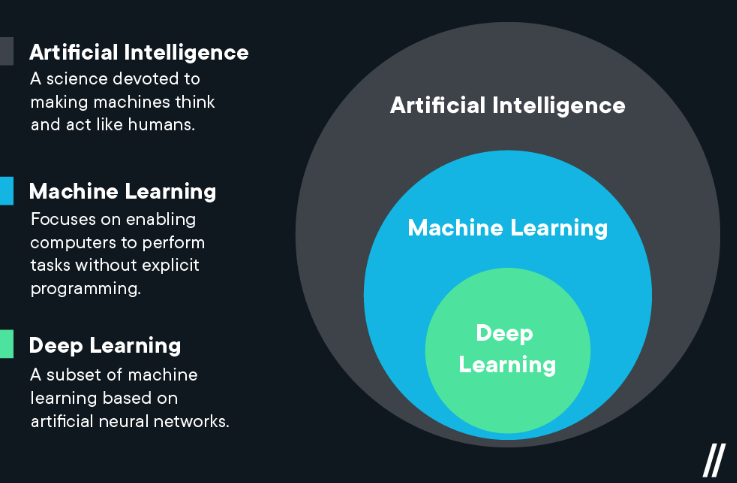
\includegraphics[width=10cm]{images/mldl.png}
    	\caption{Deep learning in the artificial intelligence domain. Courtesy of \cite{35_mldl}}
    	\label{fig:DLAI}
    \end{figure}  
    
    \section{Temporal Fusion}
    \label{sec:tempfuse}
    \section{Segmentation}
    \section{Semantic Segmentation}
    \label{sec:semseg}
    \subsection{Classical Semantic Segmentation}
    \subsection{Deep Learning based  Semantic Segmentation}
    \section{Temporal Fusion in Semantic Segmentation}
    Use as many sections as you need in your related work to group content into logical groups

    Don't forget to correctly cite your sources \cite{art1}.
    \section{Limitations of previous work}
\end{document}
